\documentclass[xcolor={table}]{beamer}
\usepackage{fleqn}
\usepackage{graphicx}
\usepackage{coordsys} %for \numbline commander

%Setup appearance:
\usetheme{Darmstadt}
\usefonttheme[onlylarge]{structurebold}
\setbeamerfont*{frametitle}{size=\normalsize,series=\bfseries}
\setbeamertemplate{navigation symbols}{}
\setbeamertemplate{bibliography item}{[\theenumiv]}

% Standard packages
\usepackage[english]{babel}
\usepackage[latin1]{inputenc}
\usepackage{times}
\usepackage[T1]{fontenc}
\usepackage{multirow}
\usepackage{subfigure}
\usepackage{pbox}
\usepackage{arydshln}
\usepackage{pifont}
\usepackage{cancel}
\usepackage{rotating} % for sideways headings

% Source Code packages
\usepackage{algorithm2e}
\usepackage{algorithmic}

\DeclareSymbolFont{extraup}{U}{zavm}{m}{n}
\DeclareMathSymbol{\varclub}{\mathalpha}{extraup}{84}
\DeclareMathSymbol{\varspade}{\mathalpha}{extraup}{85}
\DeclareMathSymbol{\varheart}{\mathalpha}{extraup}{86}
\DeclareMathSymbol{\vardiamond}{\mathalpha}{extraup}{87}

%%% This section command that adds a big page with section dividers
\usepackage{xifthen}% provides \isempty test
\newcommand{\SectionSlide}[2][]{
	\ifthenelse{\isempty{#1}}
		{\section{#2}\begin{frame} \begin{center}\begin{huge}#2\end{huge}\end{center}\end{frame}}
		{\section[#1]{#2}\begin{frame} \begin{center}\begin{huge}#2\end{huge}\end{center}\end{frame}}
}
%Extends the section slide to to include a shortened section title for the navigation bar as a second parameter
\newcommand{\SectionSlideShortHeader}[3][]{
	\ifthenelse{\isempty{#1}}
		{\section[#3]{#2}\begin{frame} \begin{center}\begin{huge}#2\end{huge}\end{center}\end{frame}}
		{\section[#1]{#2}\begin{frame} \begin{center}\begin{huge}#3\end{huge}\end{center}\end{frame}}
}

\newcommand{\refer}[1]{\footnote{#1}}
\newcommand{\GW}{\text{\textit{Guess-Who~}}}
\newcommand{\keyword}[1]{\alert{\textbf{#1}}\index{#1}}
\newcommand{\firstkeyword}[1]{\textbf{#1}\index{#1}}
\newcommand{\indexkeyword}[1]{\alert{\textbf{#1}\index{#1}}}
\newcommand{\featN}[1]{\textsc{#1}}
\newcommand{\featL}[1]{\textit{'#1'}}
 \newcommand{\ourRef}[1]{\ref{#1} $^{\text{\tiny[\pageref{#1}]}}$}
 \newcommand{\ourEqRef}[1]{\eqref{#1}$^{\text{\tiny[\pageref{#1}]}}$}
  
\DeclareMathOperator*{\argmax}{argmax}
\DeclareMathOperator*{\argmin}{argmin}

\title{Information-based Learning\\Sections $4.1, 4.2, 4.3$}
	\author{John D. Kelleher and Brian Mac Namee and Aoife D'Arcy}
	\institute{}
	\date{}
	
	
\begin{document}
\begin{frame}
	\titlepage
\end{frame}
\begin{frame}
	 \tableofcontents
\end{frame}

\begin{frame}
	\begin{itemize}
		\item In this chapter we are going to introduce a machine learning algorithm that tries to build predictive models \keyword{using only the most informative features}.
		\item In this context an informative feature is a \keyword{descriptive feature} whose values split the instances in the dataset into \keyword{homogeneous sets} with respect to the target feature value.
	\end{itemize}
\end{frame}

\SectionSlide{Big Idea}



 \begin{frame} 
\begin{figure}[htb]
	\centering
\begin{tabular}{cccc}
		\subfigure[Brian]{\includegraphics[width=0.2\textwidth]{./images/Brian.png}} &
		\subfigure[John]{\includegraphics[width=0.2\textwidth]{./images/John.png}} &
		\subfigure[Aphra]{\includegraphics[width=0.2\textwidth]{./images/Aphra.png}} &
		\subfigure[Aoife]{\includegraphics[width=0.2\textwidth]{./images/Aoife.png}}\\
	\end{tabular}
	\caption{Cards showing character faces and names for the \GW game}.
	\label{fig:guesswho}
\end{figure}
\begin{table}
\centering
\begin{footnotesize}
\begin{tabular}{c c c c }
\hline
\textbf{Man} & \textbf{Long Hair} & \textbf{Glasses} & \textbf{Name}\\
\hline
Yes & No & Yes & Brian\\
Yes & No & No & John\\
No & Yes & No & Aphra\\
No & No & No & Aoife\\
\hline
\end{tabular}
\end{footnotesize}
\label{tab:gw-domain}
\end{table}%
\end{frame} 

 \begin{frame} 
\begin{figure}[htb]
	\centering
\begin{tabular}{cccc}
		\subfigure[Brian]{\includegraphics[width=0.2\textwidth]{./images/Brian.png}} &
		\subfigure[John]{\includegraphics[width=0.2\textwidth]{./images/John.png}} &
		\subfigure[Aphra]{\includegraphics[width=0.2\textwidth]{./images/Aphra.png}} &
		\subfigure[Aoife]{\includegraphics[width=0.2\textwidth]{./images/Aoife.png}}\\
	\end{tabular}
	\caption{Cards showing character faces and names for the \GW game}.
	\label{fig:guesswho}
\end{figure}
\begin{block}{Which question would you ask first:}
\begin{enumerate}
	\item Is it a man?
	\item Does the person wear glasses?
\end{enumerate}
\end{block}
\end{frame} 

 \begin{frame} 
\begin{figure}
		\centering
\begin{footnotesize}
\begin{tabular}{cc}
		\subfigure[]{\label{fig:dectreefaces2} \includegraphics[width=0.45\textwidth]{./images/dectreefacesUs2.pdf}} &
		\subfigure[]{\label{fig:dectreefaces3} \includegraphics[width=0.45\textwidth]{./images/dectreefacesUs3.pdf}}\\
		\end{tabular}
\end{footnotesize}
	\caption{The different question sequences that can follow in a game of \GW beginning with the question \alert{Does the person wear glasses?}}
	\label{fig:dectreefaces2and3}
\end{figure}
\end{frame} 

 \begin{frame}
\begin{itemize}
	\item In both of the diagrams:
	\begin{itemize}
		\item one path is 1 question long, 
	 	\item one path is 2 questions long, 
		\item and two paths are 3 questions long.
	\end{itemize}
	\item Consequently, if you ask Question (2) first the average number of questions you have to ask per game is:
\end{itemize}
\begin{equation*}
\frac{1+2+3+3}{4}=2.25
\end{equation*}
\end{frame} 

 \begin{frame} 
\begin{figure}[htb]
		\centerline{
		\includegraphics[width=0.5\textwidth]{./images/dectreefacesUs1.pdf}
		}
	\caption{The different question sequences that can follow in a game of \GW beginning with the question \alert{Is it a man?}}
	\label{fig:dectreefaces1}
\end{figure}
\end{frame} 

 \begin{frame} 
\begin{itemize}
	\item All the paths in this diagram are two questions long. 
	\item So, on average if you ask Question (1) first the average number of questions you have to ask per game is:
\end{itemize}
\begin{equation*}
\frac{2+2+2+2}{4}=2 
\end{equation*}
\end{frame} 

\begin{frame}
	\begin{itemize}
		\item On average getting an answer to Question (1) seems to give you more information than an answer to Question (2): less follow up questions.
		\item This is not because of the literal message of the answers: YES or NO.
		\item It is to do with how the answer to each questions splits the domain into different sized sets based on the value of the descriptive feature the question is asked about and the likelihood of each possible answer to the question.
	\end{itemize}
\end{frame}

\begin{frame}
	\begin{alertblock}{Big Idea}
	\begin{itemize}
		\item So the big idea here is to figure out which features are the most informative ones to ask questions about by considering the effects of the different answers to the questions, in terms of:
		\begin{enumerate}
			\item how the domain is split up after the answer is received, 			
			\item and the likelihood of each of the answers.
		\end{enumerate} 
			\end{itemize}
	\end{alertblock}
\end{frame}

\SectionSlide{Fundamentals}

\subsection{Decision Trees}

\begin{frame}
	\begin{itemize}
		\item A decision tree consists of:
		\begin{enumerate}
			\item  a \keyword{root node} (or starting node),
			\item  \keyword{interior nodes} 
			\item and \keyword{leaf nodes} (or terminating nodes). 
		\end{enumerate}
		\item Each of the non-leaf nodes (root and interior) in the tree specifies a test to be carried out on one of the query's descriptive features. 
		\item Each of the leaf nodes specifies a predicted classification for the query. 
	\end{itemize}
\end{frame}

 \begin{frame} 
\begin{table}[!hbt]
\caption{An email spam prediction dataset.}
\label{table:spemDecTreeDataset}
\centering
\begin{footnotesize}
\begin{tabular}{ccccr}
\hline
	 & \featN{Suspicious}	& \featN{Unknown}	 & \featN{Contains}	 & \featN{} \\
\featN{ID}	 & \featN{Words}	& \featN{Sender}	 & \featN{Images}	 & \featN{Class} \\
\hline
376	 & true	 & false 	 & true	& spam \\
489	 & true	 & true 	 & false	& spam \\
541	 & true	 & true 	 & false	& spam \\
693	 & false	 & true 	 & true	& ham \\
782	 & false	 & false 	 & false	& ham \\
976	 & false	 & false 	 & false	& ham \\
\hline
\end{tabular}
\end{footnotesize}
\end{table}
\end{frame} 

 \begin{frame} 
\begin{figure}[htb]
	\centering
			\subfigure[]{\label{fig:dectreesA}\includegraphics[width=0.38\textwidth]{./images/spamdectree2_mod.pdf}}
			\subfigure[]{\label{fig:dectreesB}\includegraphics[width=0.17\textwidth]{./images/spamdectree1_mod.pdf}}
			\subfigure[]{\label{fig:dectreesC}\includegraphics[width=0.38\textwidth]{./images/spamdectree3_mod.pdf}}
	\caption{(a) and (b) show two decision trees that are consistent with the instances in the spam dataset. (c) shows the path taken through the tree shown in (a) to make a prediction for the query instance: \featN{Suspicious Words} = \featL{true}, \featN{Unknown Sender} = \featL{true}, \featN{Contains Images} = \featL{true}.}
	\label{fig:dectrees}
\end{figure}
\end{frame} 

\begin{frame}
	\begin{itemize}
		\item Both of these trees will return identical predictions for all the examples in the dataset.
		\item So, which tree should we use?
	\end{itemize}
\end{frame}

\begin{frame}
	\begin{itemize}
		\item Apply the same approach as we used in the \GW game: prefer decision trees that use less tests (shallower trees).
		\item This is an example of Occam's Razor.
	\end{itemize}
\end{frame}

\begin{frame}
\begin{alertblock}{How do we create shallow trees?}
	\begin{itemize}
		\item The tree that tests \featN{Suspicious Words} at the root is very shallow because the \featN{Suspicious Words} feature perfectly splits the data into pure groups of \featL{spam} and \featL{ham}.
		\item Descriptive features that split the dataset into pure sets with respect to the target feature provide information about the target feature.
		\item So we can make shallow trees by testing the informative features early on in the tree.
		\item All we need to do that is a computational metric of the purity of a set: \alert{entropy}
	\end{itemize}
\end{alertblock}
\end{frame}

\subsection{Shannon's Entropy Model}

\begin{frame}
	\begin{itemize}
		\item Claude Shannon's entropy model defines a computational measure of the impurity of the elements of a set.
		\item An easy way to understand the entropy of a set is to think in terms of the uncertainty associated with guessing the result if you were to make a random selection from the set.
	\end{itemize}
\end{frame}

\begin{frame}
	\begin{itemize}
		\item Entropy is related to the probability of a outcome.
			\begin{itemize}
				\item High probability $\rightarrow$ Low entropy
				\item Low probability $\rightarrow$ High entropy
			\end{itemize}
		\item If we take the \alert{log} of a probability and multiply it by -1 we get this mapping!
	\end{itemize}
\end{frame}

\begin{frame}
							\begin{block}{What is a log?}
							Remember the $log$ of $a$ to the base $b$ is the number to which we must raise $b$ to get $a$. 
							\begin{itemize}
							\item $log_{2}(0.5) = -1$ because $2^{-1} = 0.5$
							\item $log_{2}(1)=0$ because $2^{0} = 1$
							\item $log_{2}(8) = 3$ because $2^3 = 8$
							\item $log_{5}(25) = 2$ because $5^2 = 25$		
							\item $log_{5}(32) = 2.153$ because $5^{2.153} = 32$
							\end{itemize}
							\end{block}
\end{frame}



 \begin{frame} 
\begin{figure}
\centering
	\subfigure[]{\label{fig:logprobNeg}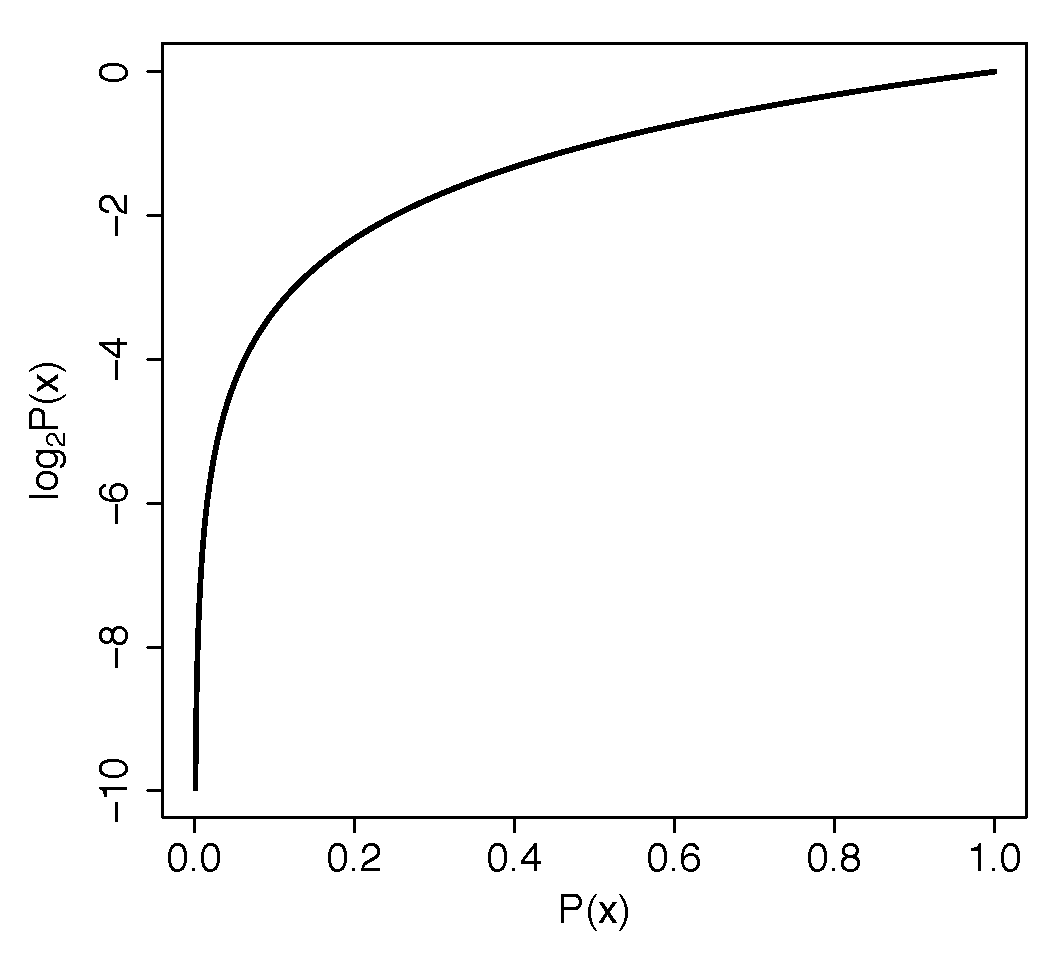
\includegraphics[width=0.4\textwidth]{./images/LogOfProbPos.pdf}}
	\subfigure[]{\label{fig:logprobPos}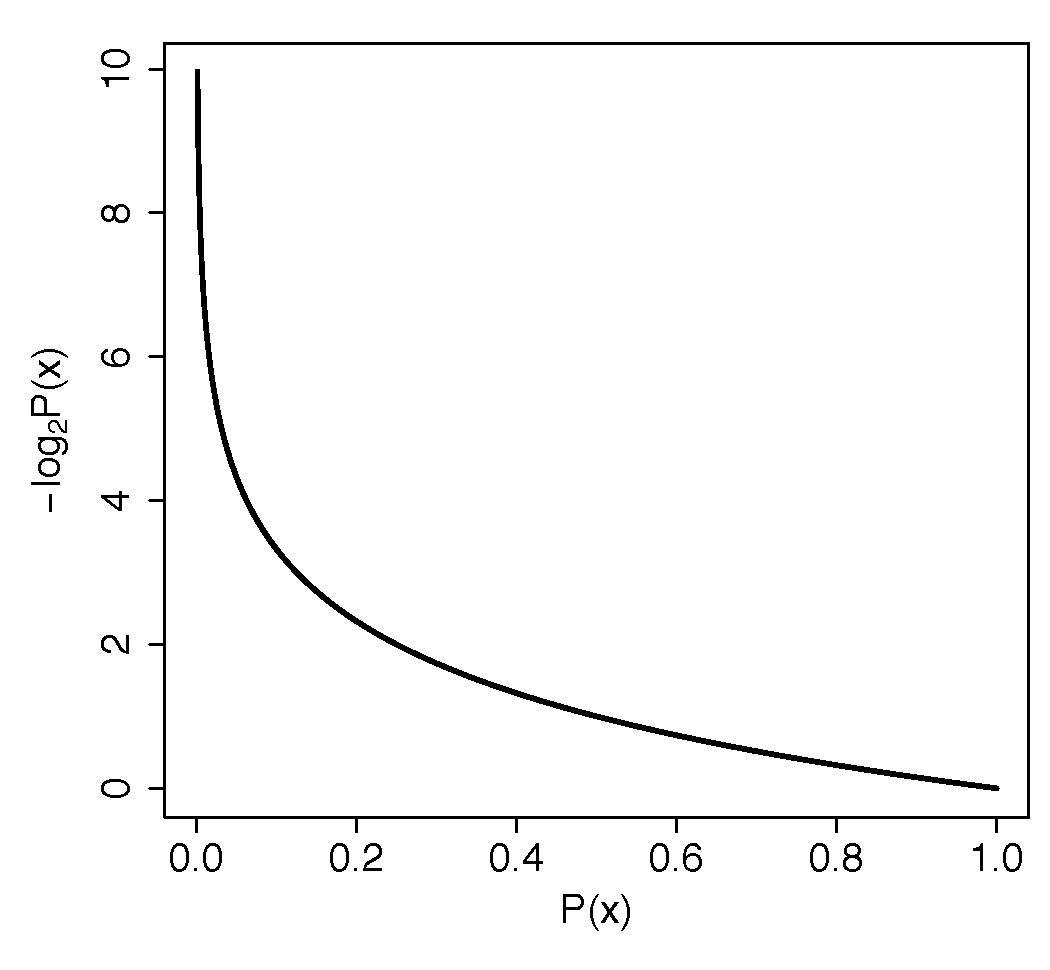
\includegraphics[width=0.4\textwidth]{./images/LogOfProbNeg.pdf}}
	\caption{(a) A graph illustrating how the value of a binary log (the log to the base 2) of a probability changes across the range of probability values. (b) the impact of multiplying these values by $-1$.}
	\label{fig:logprob}
\end{figure}
\end{frame} 

 \begin{frame} 
 \begin{itemize}
 	\item Shannon's model of entropy is a weighted sum of the logs of the probabilities of each of the possible outcomes when we make a random selection from a set.
\end{itemize}
\begin{equation}
H(t) = - \sum_{i=1}^l \left( P(t=i)\times log_s(P(t=i)) \right)
\label{eq:shannon}
\end{equation}
\end{frame} 

 \begin{frame} 
 \begin{itemize}
 	\item What is the entropy of a set of 52 different playing cards?
\end{itemize}
\begin{eqnarray*}
H(card) & = & - \sum_{i=1}^{52} P(card=i) \times log_2(P(card=i))\\
& = &  - \sum_{i=1}^{52} 0.019 \times log_2(0.019)  = - \sum_{i=1}^{52} -0.1096 \\
& = & ~ 5.700 ~ bits
\end{eqnarray*}
\end{frame} 

 \begin{frame} 
 \begin{itemize}
 	\item What is the entropy of a set of 52 playing cards if we only distinguish between the cards based on their suit $\{\varheart, \varclub, \vardiamond, \spadesuit\}$?
\end{itemize}
\end{frame}

 \begin{frame} 
\begin{eqnarray*}
	\begin{alignedat}{2}
H(suit) & =~- \sum_{l \in \{\varheart, \varclub, \vardiamond, \spadesuit\} } P(suit=l) \times log_2(P(suit=l)) \\
& =~- \big(\left( P(\varheart) \times log_2(P(\varheart)) \right) + \left( P(\varclub) \times log_2(P(\varclub)) \right) \\
  & ~~~~~~~~~~~~ + \left( P(\vardiamond) \times log_2(P(\vardiamond)) \right)  + \left( P(\spadesuit) \times log_2(P(\spadesuit)) \right)\big)\\
& =~- \big(\left(^{13}/_{52} \times log_2( ^{13}/_{52}) \right)  + \left( ^{13}/_{52} \times log_2( ^{13}/_{52} ) \right)\\
  & ~~~~~~~~~~~~ + \left(^{13}/_{52} \times log_2( ^{13}/_{52}) \right)  + \left(^{13}/_{52} \times log_2( ^{13}/_{52} ) \right)\big)\\
& =~- \big(\left(0.25 \times -2 \right)  + \left(0.25 \times -2 \right) \\
& ~~~~~~~~~~~~ + \left(0.25 \times -2 \right)  + \left(0.25 \times -2 \right)\big)\\
& =~ 2~ bits
	\end{alignedat}
\end{eqnarray*}
\end{frame} 

 \begin{frame} 
\begin{figure}
\centering
	\subfigure[$H(card)=0.00$]{\label{fig:entropyofsetsA}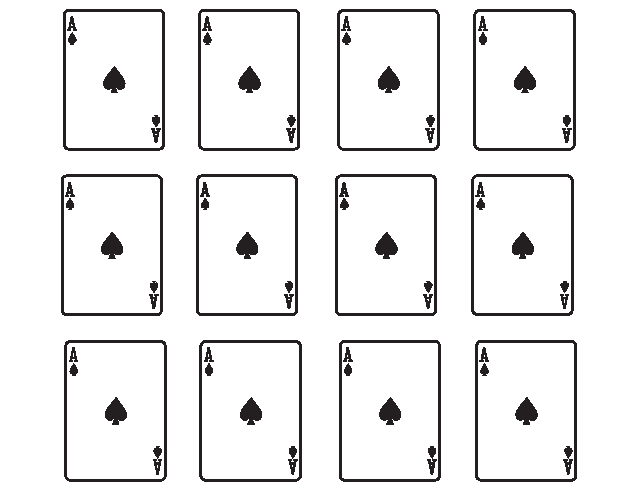
\includegraphics[width=0.32\textwidth]{./images/EntropyCardsSetA_BW.pdf}}
	\subfigure[$H(card)=0.81$]{\label{fig:entropyofsetsB}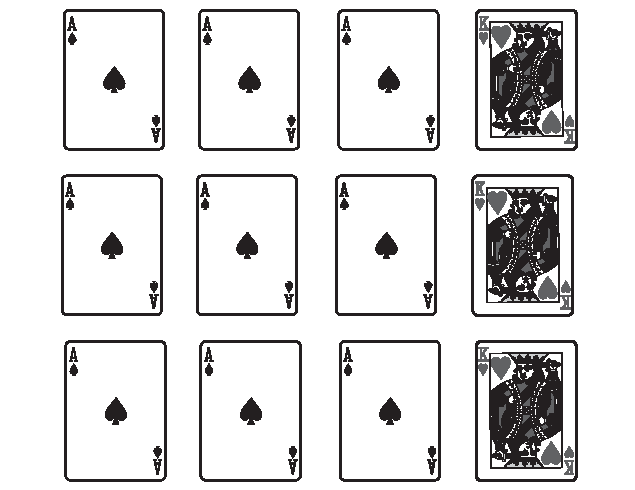
\includegraphics[width=0.32\textwidth]{./images/EntropyCardsSetB_BW.pdf}}
	\subfigure[$H(card)=1.00$]{\label{fig:entropyofsetsC}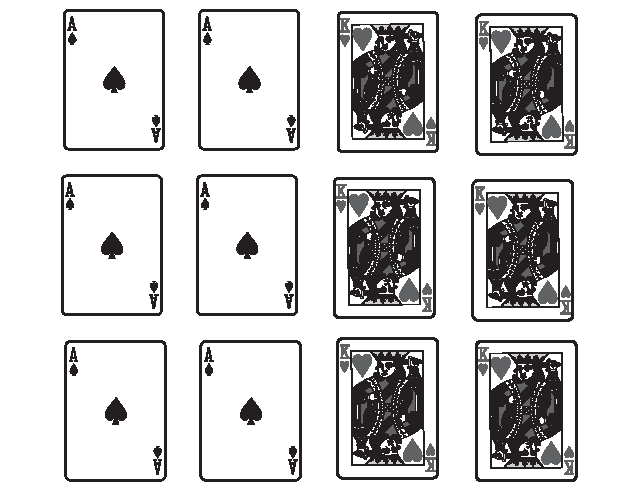
\includegraphics[width=0.32\textwidth]{./images/EntropyCardsSetC_BW.pdf}}
	\subfigure[$H(card)=1.50$]{\label{fig:entropyofsetsD}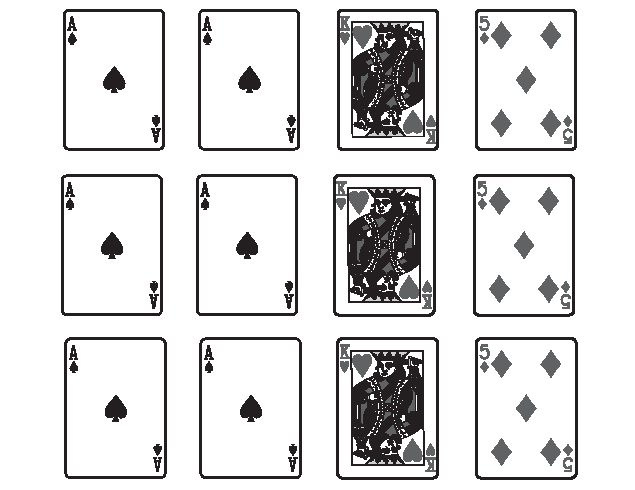
\includegraphics[width=0.32\textwidth]{./images/EntropyCardsSetD_BW.pdf}}
	\subfigure[$H(card)=1.58$]{\label{fig:entropyofsetsE}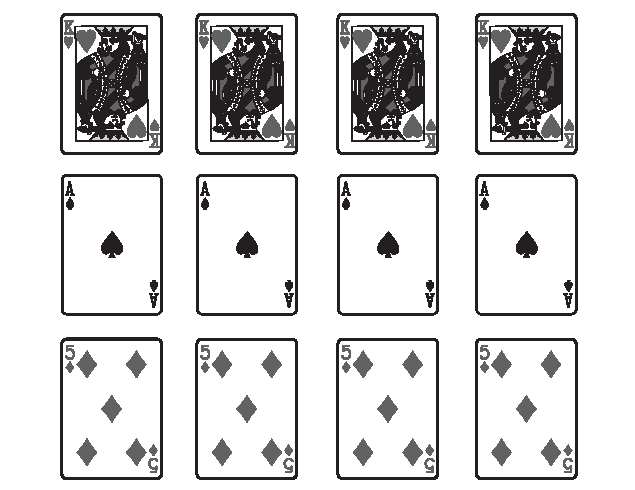
\includegraphics[width=0.32\textwidth]{./images/EntropyCardsSetE_BW.pdf}}
	\subfigure[$H(card)=3.58$]{\label{fig:entropyofsetsF}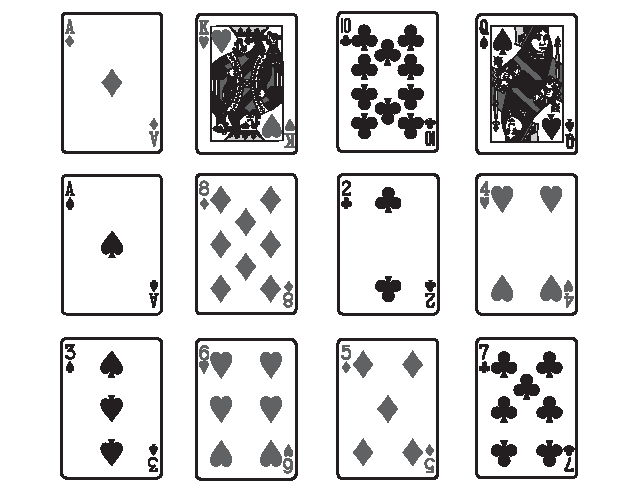
\includegraphics[width=0.32\textwidth]{./images/EntropyCardsSetF_BW.pdf}}
	\caption{The entropy of different sets of playing cards measured in bits.}
	\label{fig:entropyofsets}
\end{figure}
\end{frame} 

 \begin{frame} 
\begin{table}[!tb]
\caption{The relationship between the entropy of a message and the set it was selected from.}
\label{table:messageEntropy}
\centering
\resizebox{\textwidth}{!}{
\begin{tabular}{ l l}
\hline
\textbf{Entropy of a Message}	 & \textbf{Properties of the Message Set} \\
\hline
High         &  A large set of equally likely messages.\\ 
Medium   &   A large set of messages, some more likely than others.\\
Medium   &   A small set of equally likely messages.\\
Low	       &   A small set of messages with one very likely message.\\
\hline
\end{tabular}
}
\end{table}
\end{frame} 

\subsection{Information Gain}

 \begin{frame} 
\begin{figure}
	\centering
		\subfigure[]{\label{fig:wordsplit} \includegraphics[width=0.31\textwidth]{./images/spamham-wordsplit_mod.pdf}}
		\subfigure[]{\label{fig:sendersplit} \includegraphics[width=0.31\textwidth]{./images/spamham-sendersplit_mod.pdf}}
		\subfigure[]{\label{fig:imagessplit} \includegraphics[width=0.31\textwidth]{./images/spamham-imagesplit_mod.pdf}}
	\caption{How the instances in the spam dataset split when we partition using each of the different descriptive features from the spam dataset in Table \ourRef{table:spemDecTreeDataset}}
	\label{fig:spamhamfeaturesplits}
\end{figure}
\end{frame} 

\begin{frame}
	\begin{itemize}
		\item Our intuition is that the ideal discriminatory feature will partition the data into \textbf{pure} subsets where all the instances in each subset have the same classification. 
		\begin{itemize}
		\item \featN{Suspicious Words} perfect split. 
		\item \featN{Unknown Sender} mixture but some information (when \featL{true} most instances are \featL{spam}).
		\item \featN{Contains Images} no information.
		\end{itemize}
		\item One way to implement this idea is to use a metric called \keyword{information gain}. 
	\end{itemize}
\end{frame}

\begin{frame}
\begin{block}{Information Gain}
\begin{itemize}
	\item The information gain of a descriptive feature can be understood as a measure of the reduction in the overall entropy of a prediction task by testing on that feature. 
\end{itemize}
\end{block}
\end{frame}

 \begin{frame} 
Computing information gain involves the following 3 equations: 
\begin{equation}
H\left(t, \mathcal{D}\right) = - \sum_{l \in levels(t)} \left( P(t=l) \times log_2(P(t=l)) \right)
\label{eq:hds}
\end{equation}
\begin{equation}
rem\left(d,\mathcal{D}\right) = 
\sum_{l \in levels\left(d\right)} 
\underbrace{
\frac{|\mathcal{D}_{d=l}|}{|\mathcal{D}|}}_{\text{weighting}} \times
 \underbrace{H\left(t, \mathcal{D}_{d=l}\right)}_{
	\substack{
		\text{entropy of}\\
		\text{partition }\mathcal{D}_{d=l}
	}
}
\label{eq:ent-rem}
\end{equation}
\begin{equation}
IG\left(d,\mathcal{D}\right) = H\left(t,\mathcal{D}\right) - rem\left(d, \mathcal{D}\right)
\label{eq:info-gain}
\end{equation}
\end{frame} 

\begin{frame}
	\begin{itemize}
		\item As an example we will calculate the information gain for each of the descriptive features in the spam email dataset.
	\end{itemize}
\end{frame}

\begin{frame}
	\begin{itemize}
		\item Calculate the \alert{entropy} for the target feature in the dataset.
	\end{itemize}
	\begin{equation*}
H\left(t, \mathcal{D}\right) = - \sum_{l \in levels(t)} \left( P(t=l) \times log_2(P(t=l)) \right)
\label{eq:hds}
\end{equation*}
	\begin{table}[!hbt]
\centering
\begin{footnotesize}
\begin{tabular}{ccccr}
\hline
	 & \featN{Suspicious}	& \featN{Unknown}	 & \featN{Contains}	 & \featN{} \\
\featN{ID}	 & \featN{Words}	& \featN{Sender}	 & \featN{Images}	 & \featN{Class} \\
\hline
376	 & true	 & false 	 & true	& spam \\
489	 & true	 & true 	 & false	& spam \\
541	 & true	 & true 	 & false	& spam \\
693	 & false	 & true 	 & true	& ham \\
782	 & false	 & false 	 & false	& ham \\
976	 & false	 & false 	 & false	& ham \\
\hline
\end{tabular}
\end{footnotesize}
\end{table}
\end{frame}


 \begin{frame} 
\begin{footnotesize}
\begin{equation*}
	\begin{alignedat}{2}
H\left(t, \mathcal{D}\right) &=~-& \sum_{l \in \{\featL{spam}, \featL{ham}\}} \left( P(t=l) \times log_2(P(t=l)) \right)\\
   &=~-& ( \left(P(t=\featL{spam}) \times log_2(P(t=\featL{spam})\right)\\
 && + \left(P(t=\featL{ham}) \times log_2(P(t=\featL{ham})\right) )\\
   &=~-& \left( \left( ^3/_6 \times log_2(^3/_6)\right) + \left(^3/_6  \times log_2(^3/_6) \right) \right)\\
&=& 1~bit
	\end{alignedat}
\label{eq:hdsspam}
\end{equation*}
\end{footnotesize}
\end{frame} 

\begin{frame}
	\begin{itemize}
		\item Calculate the \alert{remainder} for the \featN{Suspicious Words} feature in the dataset.
	\end{itemize}
\begin{equation*}
rem\left(d,\mathcal{D}\right) = 
\sum_{l \in levels\left(d\right)} 
\underbrace{
\frac{|\mathcal{D}_{d=l}|}{|\mathcal{D}|}}_{\text{weighting}} \times
 \underbrace{H\left(t, \mathcal{D}_{d=l}\right)}_{
	\substack{
		\text{entropy of}\\
		\text{partition }\mathcal{D}_{d=l}
	}
}
\end{equation*}
	\begin{table}[!hbt]
\centering
\begin{footnotesize}
\begin{tabular}{ccccr}
\hline
	 & \featN{Suspicious}	& \featN{Unknown}	 & \featN{Contains}	 & \featN{} \\
\featN{ID}	 & \featN{Words}	& \featN{Sender}	 & \featN{Images}	 & \featN{Class} \\
\hline
376	 & true	 & false 	 & true	& spam \\
489	 & true	 & true 	 & false	& spam \\
541	 & true	 & true 	 & false	& spam \\
693	 & false	 & true 	 & true	& ham \\
782	 & false	 & false 	 & false	& ham \\
976	 & false	 & false 	 & false	& ham \\
\hline
\end{tabular}
\end{footnotesize}
\end{table}
\end{frame}



 \begin{frame} 
\begin{footnotesize}
\begin{equation*}
\begin{alignedat}{2}
rem&\left(\text{\featN{words}},\mathcal{D}\right)\\
&= \left(\frac{|\mathcal{D}_{\text{\featN{words}}=T}|}{|\mathcal{D}|} \times H\left(t,\mathcal{D}_{\text{\featN{words}}=T}\right) \right) + \left(\frac{|\mathcal{D}_{\text{\featN{words}}=F}|}{|\mathcal{D}|} \times H\left(t,\mathcal{D}_{\text{\featN{words}}=F}\right) \right) \\
&= \left(^3/_6 \times \left(-\sum_{l \in \{\text{\featL{spam}},\text{\featL{ham}}\}} P(t=l) \times log_2(P(t=l))\right) \right) \\
&~+ \left( ^3/_6 \times \left(-\sum_{l \in \{\text{\featL{spam}},\text{\featL{ham}}\}} P(t=l) \times log_2(P(t=l)) \right)\right)\\
&=
\left(
^3/_6 \times
\left( - \left(
\left( ^3/_3 \times log_2( ^3/_3) \right)
+
\left( ^0/_3 \times log_2( ^0/_3) \right)
\right)
\right)
\right)
\\
&~+
\left( ^3/_6 \times
\left( - \left(
\left( ^0/_3 \times log_2( ^0/_3) \right)
+
\left( ^3/_3 \times log_2( ^3/_3) \right)
\right)
\right)
\right) = 0~bits
\end{alignedat}
\label{eq:remaindersw}
\end{equation*}
\end{footnotesize}
\end{frame} 

\begin{frame}
	\begin{itemize}
		\item Calculate the \alert{remainder} for the \featN{Unknown Sender} feature in the dataset.
	\end{itemize}
\begin{equation*}
rem\left(d,\mathcal{D}\right) = 
\sum_{l \in levels\left(d\right)} 
\underbrace{
\frac{|\mathcal{D}_{d=l}|}{|\mathcal{D}|}}_{\text{weighting}} \times
 \underbrace{H\left(t, \mathcal{D}_{d=l}\right)}_{
	\substack{
		\text{entropy of}\\
		\text{partition }\mathcal{D}_{d=l}
	}
}
\end{equation*}
	\begin{table}[!hbt]
\centering
\begin{footnotesize}
\begin{tabular}{ccccr}
\hline
	 & \featN{Suspicious}	& \featN{Unknown}	 & \featN{Contains}	 & \featN{} \\
\featN{ID}	 & \featN{Words}	& \featN{Sender}	 & \featN{Images}	 & \featN{Class} \\
\hline
376	 & true	 & false 	 & true	& spam \\
489	 & true	 & true 	 & false	& spam \\
541	 & true	 & true 	 & false	& spam \\
693	 & false	 & true 	 & true	& ham \\
782	 & false	 & false 	 & false	& ham \\
976	 & false	 & false 	 & false	& ham \\
\hline
\end{tabular}
\end{footnotesize}
\end{table}
\end{frame}


 \begin{frame} 
\begin{footnotesize}
\begin{equation*}
\begin{alignedat}{2}
rem&\left(\text{\featN{sender}},\mathcal{D}\right)\\
&= \left(\frac{|\mathcal{D}_{\text{\featN{sender}}=T}|}{|\mathcal{D}|} \times H\left(t,\mathcal{D}_{\text{\featN{sender}}=T}\right) \right) + \left(\frac{|\mathcal{D}_{\text{\featN{sender}}=F}|}{|\mathcal{D}|} \times H\left(t,\mathcal{D}_{\text{\featN{sender}}=F}\right) \right) \\
&= \left(^3/_6 \times \left(-\sum_{l \in \{\text{\featL{spam}},\text{\featL{ham}}\}} P(t=l) \times log_2(P(t=l))\right) \right) \\
&~+ \left( ^3/_6 \times \left(-\sum_{l \in \{\text{\featL{spam}},\text{\featL{ham}}\}} P(t=l) \times log_2(P(t=l)) \right)\right)\\
&=
\left(
^3/_6 \times
\left( - \left(
\left( ^2/_3 \times log_2( ^2/_3) \right)
+
\left( ^1/_3 \times log_2( ^1/_3) \right)
\right)
\right)
\right)
\\
&~+
\left( ^3/_6 \times
\left( - \left(
\left( ^1/_3 \times log_2( ^1/_3) \right)
+
\left( ^2/_3 \times log_2( ^2/_3) \right)
\right)
\right)
\right) = 0.9183~bits
\end{alignedat}
\label{eq:remainderus}
\end{equation*}
\end{footnotesize}
\end{frame} 

\begin{frame}
	\begin{itemize}
		\item Calculate the \alert{remainder} for the \featN{Contains Images} feature in the dataset.
	\end{itemize}
\begin{equation*}
rem\left(d,\mathcal{D}\right) = 
\sum_{l \in levels\left(d\right)} 
\underbrace{
\frac{|\mathcal{D}_{d=l}|}{|\mathcal{D}|}}_{\text{weighting}} \times
 \underbrace{H\left(t, \mathcal{D}_{d=l}\right)}_{
	\substack{
		\text{entropy of}\\
		\text{partition }\mathcal{D}_{d=l}
	}
}
\end{equation*}
	\begin{table}[!hbt]
\centering
\begin{footnotesize}
\begin{tabular}{ccccr}
\hline
	 & \featN{Suspicious}	& \featN{Unknown}	 & \featN{Contains}	 & \featN{} \\
\featN{ID}	 & \featN{Words}	& \featN{Sender}	 & \featN{Images}	 & \featN{Class} \\
\hline
376	 & true	 & false 	 & true	& spam \\
489	 & true	 & true 	 & false	& spam \\
541	 & true	 & true 	 & false	& spam \\
693	 & false	 & true 	 & true	& ham \\
782	 & false	 & false 	 & false	& ham \\
976	 & false	 & false 	 & false	& ham \\
\hline
\end{tabular}
\end{footnotesize}
\end{table}
\end{frame}


 \begin{frame} 
\begin{footnotesize}
\begin{equation*}
\begin{alignedat}{2}
rem&\left(\text{\featN{images}},\mathcal{D}\right)\\
&= \left(\frac{|\mathcal{D}_{\text{\featN{images}}=T}|}{|\mathcal{D}|} \times H\left(t,\mathcal{D}_{\text{\featN{images}}=T}\right) \right) + \left(\frac{|\mathcal{D}_{\text{\featN{images}}=F}|}{|\mathcal{D}|} \times H\left(t,\mathcal{D}_{\text{\featN{images}}=F}\right) \right) \\
&= \left(^2/_6 \times \left(-\sum_{l \in \{\text{\featL{spam}},\text{\featL{ham}}\}} P(t=l) \times log_2(P(t=l))\right) \right) \\
&~+ \left( ^4/_6 \times \left(-\sum_{l \in \{\text{\featL{spam}},\text{\featL{ham}}\}} P(t=l) \times log_2(P(t=l)) \right)\right)\\
&=
\left(
^2/_6 \times
\left( - \left(
\left( ^1/_2 \times log_2( ^1/_2) \right)
+
\left( ^1/_2 \times log_2( ^1/_2) \right)
\right)
\right)
\right)
\\
&~+
\left( ^4/_6 \times
\left( - \left(
\left( ^2/_4 \times log_2( ^2/_4) \right)
+
\left( ^2/_4 \times log_2( ^2/_4) \right)
\right)
\right)
\right) = 1~bit
\end{alignedat}
\label{eq:remainderci}
\end{equation*}
\end{footnotesize}
\end{frame} 

\begin{frame}
	\begin{itemize}
		\item Calculate the \alert{information gain} for the three descriptive feature in the dataset.
	\end{itemize}
\begin{equation*}
IG\left(d,\mathcal{D}\right) = H\left(t,\mathcal{D}\right) - rem\left(d, \mathcal{D}\right)
\label{eq:info-gain}
\end{equation*}
\end{frame}


 \begin{frame} 
\begin{footnotesize}
\begin{equation*}
\begin{alignedat}{2}
IG\left(\text{\featN{Suspicious Words}},\mathcal{D}\right)&= H\left(\featN{Class},\mathcal{D}\right) - rem\left(\text{\featN{Suspicious Words}},\mathcal{D}\right)\\
& = 1 - 0 = 1~bit\\
	\end{alignedat}
\label{eq:infogainsw}
\end{equation*}
\begin{equation*}
\begin{alignedat}{2}
IG\left(\text{\featN{Unknown Sender}},\mathcal{D}\right)&= H\left(\featN{Class},\mathcal{D}\right) - rem\left(\text{\featN{Unknown Sender}},\mathcal{D}\right)\\
&= 1 - 0.9183 = 0.0817~bits\\
	\end{alignedat}
\label{eq:infogainus}
\end{equation*}
\begin{equation*}
\begin{alignedat}{2}
IG\left(\text{\featN{Contains Images}},\mathcal{D}\right)&= H\left(\featN{Class},\mathcal{D}\right) - rem\left(\text{\featN{Contains Images}},\mathcal{D}\right)\\
&= 1 - 1 = 0~bits\\
	\end{alignedat}
\label{eq:infogainimages}
\end{equation*}
\end{footnotesize}
\begin{itemize}
	\item The results of these calculations match our intuitions.
\end{itemize}
\end{frame} 

\SectionSlide{Standard Approach: The ID3 Algorithm}

\begin{frame}
	\begin{itemize}
		\item ID3 Algorithm (Iterative Dichotomizer 3)
		\item Attempts to create the shallowest tree that is consistent with the data that it is given.
		\item The ID3 algorithm builds the tree in a recursive, depth-first manner, beginning at the root node and working down to the leaf nodes.
	\end{itemize}
\end{frame}


\begin{frame}
\begin{enumerate}
	\item The algorithm begins by choosing the best descriptive feature to test (i.e., the best question to ask first) using \keyword{information gain}. 
	\item  A root node is then added to the tree and labelled with the selected test feature. 
	\item The training dataset is then partitioned using the test. 
	\item For each partition a branch is grown from the node. 
	\item The process is then repeated for each of these branches using the relevant partition of the training set in place of the full training set and with the selected test feature excluded from further testing. 
	\end{enumerate}
\end{frame}

\begin{frame}
The algorithm defines three situations where the recursion stops and a leaf node is constructed:
\begin{enumerate}
	\item All of the instances in the dataset have the same classification (target feature value) then return a leaf node tree with that classification as its label.
	\item The set of features left to test is empty then return a leaf node tree with the majority class of the dataset as its classification.
	\item The dataset is empty return  a leaf node tree with the majority class of the dataset at the parent node that made the recursive call. 			
\end{enumerate}
\end{frame}

\subsection{A Worked Example: Predicting Vegetation Distributions}



 \begin{frame} 
\begin{table}[h]
\caption{The vegetation classification dataset.}
\label{tab:ecologydata}
\centering
\begin{footnotesize}
\begin{tabular}{c c c c c }
\hline
\featN{ID}	 & \featN{Stream}	& \featN{Slope} & \featN{Elevation} & \featN{Vegetation}\\
\hline
1 & false & steep & high & chaparral\\
2 & true & moderate & low & riparian\\
3 & true & steep & medium & riparian\\
4 & false & steep & medium & chaparral\\
5 & false & flat & high & conifer\\
6 & true & steep & highest & conifer\\
7 & true & steep & high & chaparral\\
\hline
\end{tabular}
\end{footnotesize}
\end{table}
\end{frame} 



 \begin{frame} 
 \begin{footnotesize}
\begin{equation*}
\begin{alignedat}{2}
&H\left(\featN{Vegetation},\mathcal{D}\right)\\
&= - \sum_{l \in  \left\{ \begin{subarray}{1} \featL{chaparral}, \\ \featL{riparian}, \\ \featL{conifer} \end{subarray} \right\}} P(\featN{Vegetation}=l) \times log_2\left(P(\featN{Vegetation}=l)\right)\\
		&= -\left( \left( ^3/_7 \times log_2( ^3/_7) \right) + \left( ^2/_7  \times log_2(^2/_7)\right) + \left( ^2/_7  \times log_2(^2/_7)\right) \right)\\
		&= 1.5567~bits
	\end{alignedat}
	\label{eq:ent-hw-ds}
\end{equation*}
\end{footnotesize}

\end{frame} 



 \begin{frame} 
\begin{table}
\caption{Partition sets (Part.), entropy, remainder (Rem.) and information gain (Info. Gain) by feature for the dataset in Table \ourRef{tab:ecologydata}.}
\label{tab:splits1}
\centering
\begin{footnotesize}
\resizebox{\textwidth}{!}{
\begin{tabular}{ccccccc}
\hline
Split By &  &              &  & Partition &  & Info.\\
Feature & Level & Part. & Instances & Entropy & Rem. & Gain\\
\hline
\multirow{2}{*}{\featN{Stream}} & \featL{true} & $\mathcal{D}_1$  & $\mathbf{d}_2,\mathbf{d}_3,\mathbf{d}_6,\mathbf{d}_7$ & 1.5 & \multirow{2}{*}{1.2507} & \multirow{2}{*}{0.3060}\\
 & \featL{false} & $\mathcal{D}_2$ & $\mathbf{d}_1,\mathbf{d}_4,\mathbf{d}_5$ & 0.9183 &  & \\
\hline

\multirow{3}{*}{\featN{Slope}} & \featL{flat} & $\mathcal{D}_3$ & $\mathbf{d}_5$  & 0 & \multirow{3}{*}{0.9793} & \multirow{3}{*}{0.5774}\\
& \featL{moderate} & $\mathcal{D}_4$ & $\mathbf{d}_2$ & 0 &  & \\
& \featL{steep} & $\mathcal{D}_5$ & $\mathbf{d}_1,\mathbf{d}_3,\mathbf{d}_4,\mathbf{d}_6,\mathbf{d}_7$ & 1.3710 &  & \\

\hline
\multirow{4}{*}{\featN{Elevation}} & \featL{low} & $\mathcal{D}_6$ & $\mathbf{d}_2$  & 0 & \multirow{4}{*}{0.6793} & \multirow{4}{*}{0.8774}\\
 & \featL{medium} & $\mathcal{D}_7$ & $\mathbf{d}_3,\mathbf{d}_4$ & 1.0 &  & \\
 & \featL{high} & $\mathcal{D}_8$ & $\mathbf{d}_1,\mathbf{d}_5,\mathbf{d}_7$ & 0.9183 &  & \\
 & \featL{highest} & $\mathcal{D}_9$ & $\mathbf{d}_6$ & 0 &  & \\
\hline
\end{tabular}
}
\end{footnotesize}
\end{table}
\end{frame} 



 \begin{frame} 
\begin{figure}
\centerline{
	\includegraphics[width=1.0\textwidth]{./images/ex-hand-ecology-dectree1_mod.pdf}
}
\caption{The decision tree after the data has been split using \featN{Elevation}.}
\label{fig:ex-hand-dectree1}
\end{figure}
\end{frame} 



 \begin{frame} 
 \begin{footnotesize}
\begin{equation*}
	\begin{alignedat}{2}
&H\left(\featN{Vegetation},\mathcal{D}_7\right)\\
&= - \sum_{l \in  \left\{ \begin{subarray}{1} \featL{chaparral}, \\ \featL{riparian}, \\ \featL{conifer} \end{subarray} \right\}} P(\featN{Vegetation}=l) \times log_2\left(P(\featN{Vegetation}=l)\right)\\
		&= -\left( \left( ^1/_2 \times log_2(^1/_2) \right) + \left(^1/_2  \times log_2(^1/_2) \right) + \left(^0/_2  \times log_2(^0/_2) \right) \right)\\
		&= 1.0~bits 	
	\end{alignedat}
	%\caption{The calculation of the entropy for the $\mathcal{D}_3$ dataset in Figure \ourRef{fig:ex-hand-dectree1}.}
	\label{eq:ent-D7}
\end{equation*}
\end{footnotesize}
\end{frame} 



 \begin{frame} 
\begin{table}
\caption{Partition sets (Part.), entropy, remainder (Rem.) and information gain (Info. Gain) by feature for the dataset $\mathcal{D}_7$ in Figure \ourRef{fig:ex-hand-dectree1}.}
\label{tab:splits2}
\centering
\begin{footnotesize}
\resizebox{\textwidth}{!}{
\begin{tabular}{ccccccc}
\hline
Split By &  &              &  & Partition &  & Info.\\
Feature & Level & Part.  & Instances & Entropy & Rem. & Gain\\
\hline
\multirow{2}{*}{\featN{Stream}} & \featL{true} & $\mathcal{D}_{10}$  & $\mathbf{d}_3$  & 0 & \multirow{2}{*}{0} & \multirow{2}{*}{1.0}\\
 & \featL{false} & $\mathcal{D}_{11}$ & $\mathbf{d}_4$  & 0 &  & \\
\hline
\multirow{3}{*}{\featN{Slope}} & \featL{flat} & $\mathcal{D}_{12}$ & ~  & 0 & \multirow{3}{*}{1.0} & \multirow{3}{*}{0}\\
& \featL{moderate} & $\mathcal{D}_{13}$ & ~ & 0 &  & \\
& \featL{steep} & $\mathcal{D}_{14}$ & $\mathbf{d}_3,\mathbf{d}_4$ & 1.0 &  & \\
\hline
\end{tabular}
}
\end{footnotesize}
\end{table}
\end{frame} 



 \begin{frame} 
\begin{figure}
\centerline{
	\includegraphics[width=\textwidth]{./images/ex-hand-ecology-dectree2_mod.pdf}
}
\caption{The state of the decision tree after the $\mathcal{D}_7$ partition has been split using \featN{Stream}.}
\label{fig:ex-hand-dectree2}
\end{figure}
\end{frame} 



 \begin{frame} 
 \begin{footnotesize}
\begin{equation*}
	\begin{alignedat}{2}
&H\left(\featN{Vegetation},\mathcal{D}_8\right)\\
&= - \sum_{l \in  \left\{ \begin{subarray}{1} \featL{chaparral}, \\ \featL{riparian}, \\ \featL{conifer} \end{subarray} \right\}} P(\featN{Vegetation}=l) \times log_2\left(P(\featN{Vegetation}=l)\right)\\
		&= -\left( \left( ^2/_3 \times log_2(^2/_3) \right) + \left(^0/_3  \times log_2(^0/_3) \right) + \left(^1/_3  \times log_2(^1/_3) \right) \right)\\
		&= 0.9183~bits 	
	\end{alignedat}
	%\caption{The calculation of the entropy for the $\mathcal{D}_3$ dataset in Figure \ourRef{fig:ex-hand-dectree1}.}
	\label{eq:ent-D8}
\end{equation*}
\end{footnotesize}
\end{frame} 

 \begin{frame} 
\begin{table}
\caption{Partition sets (Part.), entropy, remainder (Rem.) and information gain (Info. Gain) by  by feature for the dataset $\mathcal{D}_8$ in Figure \ourRef{fig:ex-hand-dectree2}.}
\label{tab:splits3}
\centering
\begin{footnotesize}
\resizebox{\textwidth}{!}{
\begin{tabular}{ccccccc}
\hline
Split By &  &              &  & Partition &  & Info.\\
Feature & Level & Part.  & Instances & Entropy & Rem. & Gain \\
\hline
\multirow{2}{*}{\featN{Stream}} & \featL{true} & $\mathcal{D}_{15}$  & $\mathbf{d}_7$  & 0 & \multirow{2}{*}{0.6666} & \multirow{2}{*}{0.2517}\\
 & \featL{false} & $\mathcal{D}_{16}$ & $\mathbf{d}_1,\mathbf{d}_5$  & 1.0 &  & \\
\hline
\multirow{3}{*}{\featN{Slope}} & \featL{flat} & $\mathcal{D}_{17}$ & $\mathbf{d}_5$  & 0 & \multirow{3}{*}{0} & \multirow{3}{*}{0.9183}\\
& \featL{moderate} & $\mathcal{D}_{18}$ & ~ & 0 &  & \\
& \featL{steep} & $\mathcal{D}_{19}$ & $\mathbf{d}_1,\mathbf{d}_7$ & 0 &  & \\
\hline
\end{tabular}
}
\end{footnotesize}
\end{table}
\end{frame} 



 \begin{frame} 
\begin{figure}
\centerline{
	\includegraphics[width=\textwidth]{./images/ex-hand-ecology-dectree3_mod.pdf}
}
\caption{The state of the decision tree after the $\mathcal{D}_8$ partition has been split using \featN{Slope}.}
\label{fig:ex-hand-dectree3}
\end{figure}
\end{frame} 



 \begin{frame} 
\begin{figure}
\centerline{
	\includegraphics[width=0.8\textwidth]{./images/ex-hand-ecology-dectree4_mod.pdf}
}
\caption{The final vegetation classification decision tree.}
\label{fig:ex-hand-dectree4}
\end{figure}
\end{frame} 

\begin{frame}
\centerline{
	\includegraphics[width=0.8\textwidth]{./images/ex-hand-ecology-dectree4_mod.pdf}
}
\begin{itemize}
	\item What prediction will this decision tree model return for the following query?
\end{itemize}
\begin{center}
\featN{Stream} = \featL{true}, \featN{Slope}=\featL{Moderate}, \featN{Elevation}=\featL{High}
\end{center}
\end{frame}

\begin{frame}
\centerline{
	\includegraphics[width=0.8\textwidth]{./images/ex-hand-ecology-dectree4_mod.pdf}
}
\begin{itemize}
	\item What prediction will this decision tree model return for the following query?
\end{itemize}
\begin{center}
\featN{Stream} = \featL{true}, \featN{Slope}=\featL{Moderate}, \featN{Elevation}=\featL{High}
\end{center}
\begin{center}
\alert{\featN{Vegetation} = \featL{Chaparral}}
\end{center}
\end{frame}

\begin{frame}
\begin{table}[h]
\centering
\begin{footnotesize}
\begin{tabular}{c c c c c }
\hline
\featN{ID}	 & \featN{Stream}	& \featN{Slope} & \featN{Elevation} & \featN{Vegetation}\\
\hline
1 & false & steep & high & chaparral\\
2 & true & moderate & low & riparian\\
3 & true & steep & medium & riparian\\
4 & false & steep & medium & chaparral\\
5 & false & flat & high & conifer\\
6 & true & steep & highest & conifer\\
7 & true & steep & high & chaparral\\
\hline
\end{tabular}
\end{footnotesize}
\end{table}
\begin{center}
\featN{Stream} = \featL{true}, \featN{Slope}=\featL{Moderate}, \featN{Elevation}=\featL{High}
\end{center}
\begin{center}
\alert{\featN{Vegetation} = \featL{Chaparral}}
\end{center}
	\begin{itemize}
		\item This is an example where the model is attempting to \alert{generalize} beyond the dataset.
		\item Whether or not the generalization is correct depends on whether the assumptions used in generating the model (i.e. the \alert{inductive bias}) were appropriate.
	\end{itemize}
\end{frame}


\SectionSlide{Summary}


\begin{frame}
	\begin{itemize}
		\item The ID3 algorithm works the same way for larger more complicated datasets.
		\item There have been many extensions and variations proposed for the ID3 algorithm:
			\begin{itemize}
				\item using different impurity measures (Gini, Gain Ratio)
				\item handling continuous descriptive features
				\item to handle continuous targets
				\item pruning to guard against over-fitting
				\item using decision trees as part of an ensemble (Random Forests)
			\end{itemize}
		\item We cover these extensions in Section $4.4$.
	\end{itemize}
\end{frame}

\begin{frame}
	\tableofcontents
\end{frame}

\end{document}
